% flashcards-title: Plant height data with a straight model line across eight weeks
% flashcards-desc: Graph of height in centimeters against age in weeks. Measured points sit at week one five centimeters, week two eight, week three eleven, week four fourteen, week five seventeen, week six about nineteen and a half, week seven about twenty and a half, and week eight twenty-one. A straight model line labeled H equals two plus three times w passes upward across the full width of the graph.
\documentclass[dvisvgm,tikz,border=8pt]{standalone}
\usepackage{tikz}
\usetikzlibrary{arrows.meta,calc,positioning}
\definecolor{DeckInk}{HTML}{172A3A}
\definecolor{DeckAccent}{HTML}{176B87}
\definecolor{DeckWarm}{HTML}{D97706}
\definecolor{DeckMuted}{HTML}{667784}
\definecolor{DeckPaper}{HTML}{F7FAFC}
\tikzset{
  every node/.style={font=\sffamily, text=DeckInk},
  object/.style={draw=DeckInk, line width=1.1pt, fill=DeckPaper},
  primary/.style={draw=DeckAccent, line width=1.5pt},
  boundary/.style={draw=DeckAccent, line width=1.5pt, dashed, rounded corners=6pt},
  guide/.style={draw=DeckMuted, line width=0.9pt, dashed},
  dimension/.style={{Stealth[length=3.2mm,width=2.2mm]}-{Stealth[length=3.2mm,width=2.2mm]}, draw=DeckWarm, line width=1.2pt},
  motion/.style={-{Stealth[length=3.5mm,width=2.5mm]}, draw=DeckAccent, line width=1.5pt, dashed},
}

\begin{document}
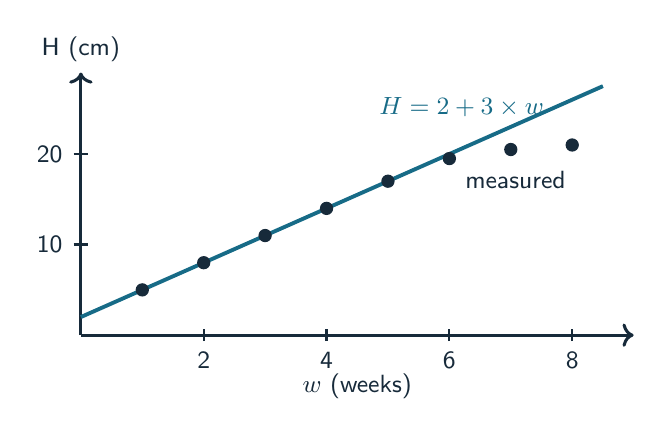
\begin{tikzpicture}[x=0.78cm, y=0.115cm]
  % Axes
  \draw[object, ->] (0,0) -- (9.0,0);
  \node[below, font=\sffamily\small] at (4.5,-3.2) {$w$ (weeks)};
  \draw[object, ->] (0,0) -- (0,29) node[above, font=\sffamily\small] {H (cm)};
  \foreach \x in {2,4,6,8} {
    \draw[DeckInk, line width=0.8pt] (\x,-0.65) -- (\x,0.65);
    \node[below, font=\sffamily\small] at (\x,-0.8) {\x};
  }
  \foreach \y in {10,20} {
    \draw[DeckInk, line width=0.8pt] (-0.12,\y) -- (0.12,\y);
    \node[left, font=\sffamily\small] at (-0.14,\y) {\y};
  }
  % Model line across the full width
  \draw[DeckAccent, line width=1.4pt] (0,2) -- (8.5,27.5);
  \node[font=\sffamily\small, text=DeckAccent, anchor=west] at (4.7,25.2)
    {$H = 2 + 3 \times w$};
  % Measured points
  \foreach \x/\y in {1/5, 2/8, 3/11, 4/14, 5/17, 6/19.5, 7/20.5, 8/21} {
    \fill[DeckInk] (\x,\y) circle [radius=2.4pt];
  }
  \node[font=\sffamily\small, anchor=north west] at (6.1,19.2) {measured};
\end{tikzpicture}
\end{document}
